\documentclass[conference]{IEEEtran}
%\documentclass[11pt,letterpaper,notitlepage, onecolumn,conference]{IEEEtran}
%\IEEEoverridecommandlockouts
% The preceding line is only needed to identify funding in the first footnote. If that is unneeded, please comment it out.
\usepackage{cite}
\usepackage{amsmath,amssymb,amsfonts}
\usepackage{algorithmic}
\usepackage{graphicx}
\usepackage{textcomp}
\usepackage{xcolor}
\usepackage{float}
\def\BibTeX{{\rm B\kern-.05em{\sc i\kern-.025em b}\kern-.08em
    T\kern-.1667em\lower.7ex\hbox{E}\kern-.125emX}}
\begin{document}

\title{ECE 471: Word and Symbol Spotting\\
}

\author{\IEEEauthorblockN{Geena Smith}
\IEEEauthorblockA{\textit{Faculty of Engineering} \\
\textit{University of Victoria}\\
Victoria, Canada \\
gmsmith@uvic.ca \\
V00835915}
\and
\IEEEauthorblockN{Joshua McIntosh}
\IEEEauthorblockA{\textit{Faculty of Engineering} \\
\textit{University of Victoria}\\
Victoria, Canada \\
jmcintosh@uvic.ca \\
V00875715}
}

\maketitle

\section{Project Description \& Scope}
The paper that we decided to base our project on \emph{Word and Symbol Spotting Using Spatial Organization of Local Descriptors}, by Marcal Rusinol and Josep Llados, proposes a method to identify both text and graphical symbols in a set of diagrams \cite{b1}. As stated by the authors, a large amount of effort is being made to digitize documents that are originally in paper form. 

At the time it was written, there were existing techniques to identify text or symbols within a document, but not at the same time without first having to separate the two. Word spotting techniques usually rely on the fact that text strings are one-dimensional structures and language has an underlying composition. Symbol spotting uses the fact that symbols usually consist of uniform regions that are highly structured. Since word spotting and symbol spotting rely on these different assumptions, neither technique would work to identify both text and symbols at the same time. 

Rusinol and Llados are very clear in their paper that they are not intending to identify both text and symbols with the great level of accuracy that dedicated methods would. Instead, they intend to propose a new technique that allows for detection without first having to separate the two, and do so with performance that is sufficient for most applications.

In our project, we are implementing the paper's proposed solution, and by doing so, we intend to verify that Rusinol and Llados' solution gives some reasonable results. We will also be using a different data set than used in the paper, which was automotive wiring diagrams, in order to show that the proposed technique applies to contexts outside of the data set used.
 

\section{Paper Overview}
Rusinol and Llados proposed a solution inspired by standard symbol spotting and object recognition methods in order to detect both text and symbols. Their solution leans on existing methods to calculate keypoints and local descriptors before branching off with their own method for indexing the descriptors.

Rusinol and Llados method for symbol spotting begins with the Harris-Laplace detector, given by Mikolajczk and Schmid \cite{b2}, to extract keypoints from the image. While other methods for extracting interest points exist, Rusinol and Llados concluded that it would not be necessary to account for affine deformations for the documents in their dataset, unlike other real images, as those deformations would not appear in the technical documents in their dataset. Harris-Laplace also automatically selects the scale of the region to which the local descriptor of the region will be computed. As details for the Harris-Laplace method are given by Mikolajczk and Schmid, implementation details were not provided. From there, the local descriptor is computed, centered on the interest points, using "off-the-shelf" descriptors. Rusinol and Llados experimented with several of these "off-the-shelf" descriptors, including SIFT features, shape contexts, Hu's geometric moment invariants, and steerable filters \cite{b1}. For our proposal, we will not examine the performance of these descriptors and base the one we use off of their findings.

Next, Rusinol and Llados propose a novel solution for matching the model descriptors with the computed image descriptors; using an indexing structure to organize descriptors, such as a hash function. As the focus of their paper is performance over accuracy, it would not be feasible to brute-force the model descriptors against the large quantity of computed descriptor and instead settle for efficiently gathering interest points similar to the model query \cite{b1}.

\begin{figure}[htbp]
	\centerline{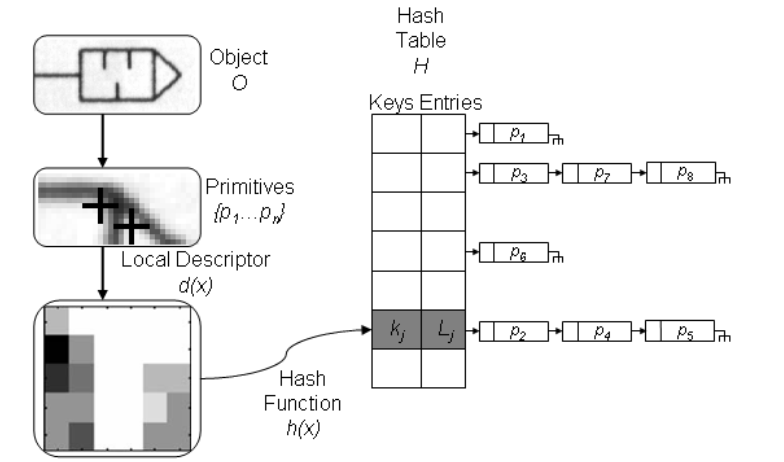
\includegraphics[width=0.8\columnwidth]{fig1.png}}
	\caption{Overview of the organization of keypoint extraction and local descriptors \cite{b1}}
	\label{Figure 1}
\end{figure}

As seen in Figure 1, the n-dimensional space of each descriptor is put into the hash table and is stored as a list for easy recovery. This list contains all keypoints with the same index, and thus have similar descriptions. Thus, the keypoints from the model image in question can also be hashed, which then will generate a list of similar keypoints.

The final step is to match the spatial organization of points from the image to those of the target model, which when combined with the efficient retrieval of locations from the hash table will be sufficient in defining similar segments in the image. A proximity graph is constructed by connecting each keypoint with $k$ of their nearest neighbors. A specific value for $k$ was not given, but an example figure from the paper shows a proximity graph of $k=5$ \cite{b1}, which will be the value we will begin with and experiment accordingly. Every pair of keypoints from the model that are connected by an edge are used for the basis of a Hough transform, in which a hypothetical center $hc$ is computed, representing a basis to be queried. Finally, the queried hypothetical centers create a voting mechanism to which keypoints with locations with the most similar descriptions and similar spatial organization are retrieved.

\section{Evaluation \& Dataset}

To communicate the experimental results, the paper utilized two measurements: precision and recall. Precision measures how well the system is able to include only relevant items in the results. 100 percent precision would mean every symbol or word that was detected is the desired symbol or word (limits false positives). Recall is the system's effectiveness in retrieving items, and a 100 percent recall would mean that every symbol or word is detected, but additional symbols or words may also be included in the result. 

To help convey these concepts, Rusinol and Llados give an example of the results retrieved when looking for a single graphical symbol or word in an image from their data set. In both the symbol and word case, all of the instances of the symbol and word are retrieved, with some false positives. This demonstrates 100 percent recall, but a lesser precision for that singular example. To explain the false positives, or lower precision, the authors give the reasoning that the falsely detected symbols have common features to the desired symbol or word, such as sharing common subparts in the case of symbols, or common prefixes or suffixes in the case of words. This reasoning seems to be rational, and the high recall, lower precision aligns with the goal of the paper: to identify both text and graphical symbols with some reliability.

The other main form that Rusinol and Llados use to convey their experimental results is in average precision and recall plots. Since the technique uses “off the shelf” local descriptors, the authors plot the average precision and recall for each of the four descriptors they tested in order to compare how the choice in descriptor affects the performance of the system. As stated in the paper, simpler descriptors have a very high precision for low recall, but the precision quickly falls as the recall increases due to the descriptors being very sensitive to differences in the same object. More complex descriptors provide a higher recall at the expense of a lower precision, meaning object detection is much better but results in more false positives. The other average precision and recall plot included in the paper is one which consists of the response for querying only text or only graphical symbols. Comparing both plots, the results of the technique to detect both symbols and text follows a very similar trend to detecting symbol or text only, despite the descriptor used. By comparing the two plots, it is very clear that the technique proposed in the paper yields successful results in detecting both symbols and text in an image with some reliability.

Although the results that were presented in the paper seemed promising, the authors failed to convey some important information about their data set. In their experiment, Rusinol and Llados use a data set which consisted of ten 3500 by 2500 pixel images from automotive wiring diagrams. From these images, they queried six objects (3 graphic symbols and 3 words). The paper showed a single example image, but they failed to communicate how similar the ten images were to each other. If the images had a high level of similarity (eg. all came from the same cumulative document or author), the results could appear more promising than if they had been run on a set of more varied images. Along a similar school of thought, the authors did not communicate which symbols or words were chosen to be queried. Symbols and words that have very similar structures would likely result in a very high recall but low precision. Finally, the number of images in the sample is very small, and could limit the reproducibility of similar results, especially when combined with the previous drawbacks associated with the data set.

In our project, we are proposing to use a data set consisting of assembly instructions from home furniture, such as is shown in Figure 2 \cite{b3}. We propose to have roughly 15 images, taken from A4 sized pdfs that have been converted to images of size 1654 by 2197 pixels. When querying the images, we hope to look at 3-5 each of symbols and words.

\begin{figure}[htbp]
	\centerline{
\includegraphics[width=0.9\columnwidth]{fig2.png}}
	\caption{Sample instruction manual to be used in the dataset \cite{b3}}
	\label{Figure 2}
\end{figure}

These instruction sets commonly consist of written instructions as well as symbols, such as for screws, dowels, or wooden pieces. We felt the symbols included in the diagrams were particularly interesting and will further test the paper's technique. For example, a top-down view of screw heads will have similar structures but could vary depending on if the screw is Phillips head, flat head, etc. We would expect the recall to be high in this case, but would be interested in the precision of the technique. Another example is with the wooden components of the furniture, such as the sides and bottoms of an item. The overall structure is very simple, but the orientation or size of the symbol would be testing the recall abilities of the technique.

\begin{thebibliography}{00}
\bibitem{b1} M. Rusinol and J. Lladnos. ``Word and symbol spotting using spatial organization of local descriptors,'' 2008 The Eighth IAPR International Workshop on Document Analysis Systems, 2008.
\bibitem{b2} K. Mikolajczyk and C. Schmid. Scale \& affine invariant interest point detectors. International Journal of ComputerVision, 60(1):63–86, 2004.
\bibitem{b3} 6 Drawer Dresser Assembly Instructions, Delta Children, New York, NY, 2014. Accessed on: January, 30, 2020. [Online]. Available: https://images-na.ssl-images-amazon.com/images/I/C13t\%2B1TH9tS.pdf
\end{thebibliography}

\end{document}
